\documentclass{article}

\usepackage[pdftex]{graphicx}
\usepackage{float}

\usepackage[utf8]{inputenc}
\usepackage{hyperref}

\title{\textbf{SDN Overlay Network with VCL and \\Open vSwitch}}
\date{\today}
%Add your name in place of your handle
\author{\textbf{Team 9} \\Kushagra Mishra : Lead\\
B Shravan Achar : Vice Lead \\ Yogesh Lele \\ Muchen Zhang \\ Gokkulasudan Rathnakumar\\ \textit{North Carolina State University}}


\begin{document}

\maketitle
\pagebreak
\tableofcontents
\pagebreak
\listoffigures
\listoftables
%TODO : independent index (aka ToC) (After completion of the report) for pages, graphs, tables.
%TODO : Each section of a new page after the completion of the report.
% list full names of all team members
\newpage

\section{Abstract}
%{The infrastructure basically contains compute, storage and networking hardware. ---- Can we add HPC compute nodes as well}
Apache VCL is an open-source system used to dynamically provision and broker remote access to a dedicated compute environment for an end-user \cite{vcl}. Setting up and maintaining VCL for a large institution like NCSU, requires large scale infrastructure. The infrastructure basically contains compute, storage and networking hardware. Managing a large virtual environment at scale grows in complexity as demand for VCL services increase. SDN helps network administrators to easily configure networking devices in a dynamic environment, where requirements are changed on a regular basis. Currently, VCL uses Linux bridges over KVM to communicate between VMs. The project aims to replace this infrastructure and use Open vSwitch(OVS) instead. With OVS running on all networking devices, it will be possible to control them using a SDN controller. This will ease the process of configuring multiple networking devices.

%Guys, we should add this below section


\section{Introduction}
% This includes problem statement (5 points), motivation
% (1 points), issues (4 points) and environment (4 points). This section should
% include references (in bibliographic form) (1 points). Problem description
% may include graphs, tables, and other types of diagrams. This section is
% intended to tell the reader what the project was about, and where it fits in the
% cloud computing world, i.e., a briefly what and why of the project.

\subsection{Problem Statement}

This project involves configuring several KVM hypervisors within VCL to use Open vSwitch and VxLAN protocol to establish a SDN overlay network among the VCL nodes. After establishing the overlay network, an openflow controller needs to be added to the SDN overlay. This provides a more complex control of the network. VCL sandboxes will be used to effectively establish a small VCL cluster running within the NCSU production VCL system.

Currently, the KVM hypervisors are using Linux bridges to connect the VMs to the host’s physical networks. This project would replace those bridges with Open vSwitches.  Additionally, tunnels between the hypervisors would be created to establish a single private network for the project VCL cluster. After the private network has been created a single management node will be used to provision VMs on all the VCL sandboxes.

\subsection{Motivation}
In the present VCL environment, suppose a user wants to configure network for 10 VCL sandboxes (analogous to single tenant having VMs spanning across multiple DataCenters). The user will have to access each sandbox to manage or make changes to the network configuration. This is cumbersome and also takes a lot of time.

The project aims to simplify this process by creating an overlay network using open vSwitch on VCL sandboxes and using a single SDN controller to manage the network. 

% \subsection{Issues}
% The networking of VCL sandboxes 


\section{Requirements}
\subsection{Functional Requirements}
\begin{enumerate}
    \item To replace the Linux bridge with open vSwitch on KVM inside a VCL Sandbox 2.4.2. After the bridge has been replaced, VCL should be able to provision VMs on the hypervisor, as it did before changing to Open vSwitch. Also, the networking changes should be persistent across reboots.

    \item To replicate the environment mentioned above on another VCL sandbox. 
    
    \item To establish a tunnel between the sandboxes running Open VSwitch and setup a private network using either VxLan or Geneve tunnelling protocol.

    \item The management node on one VCL sandbox (master) should be able to provision VMs on all such sandboxes (slaves) over the earlier described private network. For this, a single common DHCP server running on the master sandbox must be used to provide IP addresses to VMs on all sandboxes. Users must still be able to connect to a reserved VM on any sandbox, as they did before the tunnel was established.
    
    \item To reconfigure the VCL sandboxes to use a single NAT host, preferably on the master sandbox. Thus, users should be able to connect to VMs on either host. However, all connections should be made through the public IP of only one host.

    
    % After completing step 1, you will have a single sandbox working that is using
    % Open vSwitch.  So, what will be the other endpoint for the tunnel described in
    % step 2?  You need to move part of what you have in step 3 to before step 2
    % (the part about replicating the environment).
    
    % You will need to modify DHCP for the private network.
    
    % Also, note that at this point you should have replaced both bridges in the
    % sandboxes with Open vSwitches, but you are only establishing a tunnel for the
    % private network.

        
    \item To install a SDN controller on one of the sandboxes to orchestrate Open VSwitches on all the sandboxes and police the traffic over the private network.
    
\end{enumerate}

\subsection{Non-Functional Requirements}
    \begin{enumerate}
        \item To analyze and mitigate known vulnerabilities and threats introduced by the migration to OvS.
        \item To analyze performance of the entire system after introducing SDN / OvS.
        \item To analyze scaling issues introduced by OvS and tunneling.
        \item To provide succinct documentation/scripts needed for a VCL administrator to replicate these setups without having to do additional research on what commands to run and how to configure things. 
    
    \end{enumerate}
    % Use of single NAT also limits scalability (port number / FDs). NAT host is overloaded, which might limit scalability
    % Possible solutions - Use load balancer infront of a NAT. Distributed NAT service.
    
\section{System Environment}
\begin{itemize}
    \item \textbf{VCL Sandbox 2.4.2}
    \item \textbf{KVM/QEMU}
    \item \textbf{CentOS 7}
    \item \textbf{Open vSwitch}P
    \item \textbf{VxLan}
    \item \textbf{Open Daylight Controller}
\end{itemize}


\section{Design}

\begin{figure}[H]
\centering
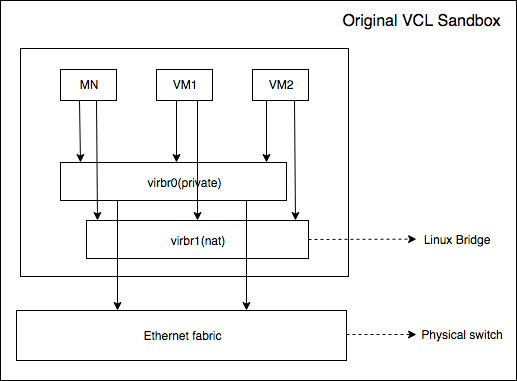
\includegraphics[width=0.9\textwidth]{vcl_linux_sandbox}
\caption{VCL sandbox with Linux Bridge}
\label{fig:allvsi}
\end{figure}

\begin{figure}[H]
\centering
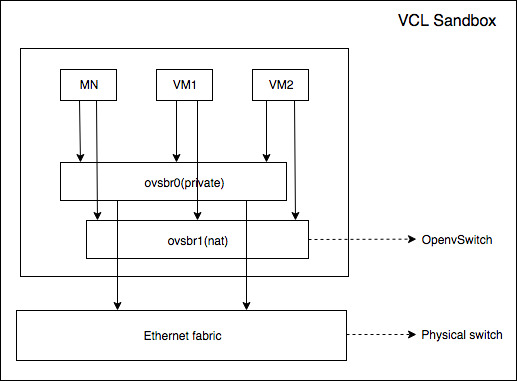
\includegraphics[width=0.9\textwidth]{vcl_ovs_sandbox}
\caption{VCL sandbox with Open vSwitch}
\label{fig:allvsi}
\end{figure}

\begin{figure}[H]
\centering
\includegraphics[width=0.9\textwidth]{vxlan_sandboxes}
\caption{VxLan tunnel between two VCL Sandbox}
\label{fig:allvsi}
\end{figure}


\begin{figure}[H]
\centering
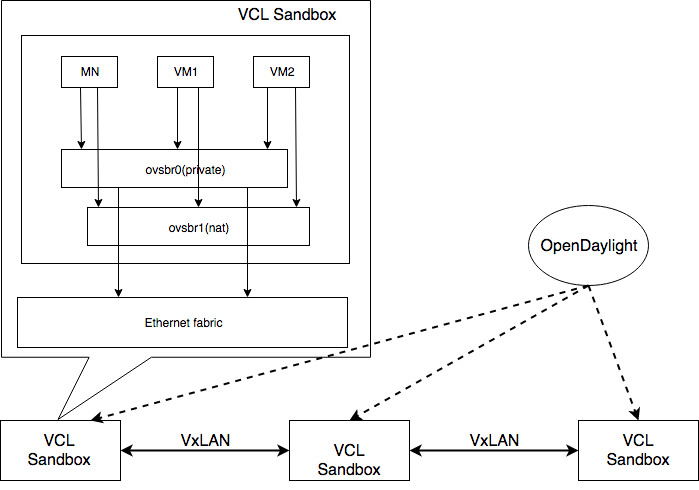
\includegraphics[width=0.9\textwidth]{Connected_vcl_sandboxes}
\caption{VCL Cluster with a single SDN Controller}
\label{fig:allvsi}
\end{figure}

\section{Implementation}
\section{Results}
\section{Verification and Validation}
%{The start up time for a host having Linux Bridges and Open v Switch bridges has not been validated. The reason is because we were provided with a pre booted up production machines to work on.}

%{Need to check the ping rate and external access to the VM}
\begin{tabular}{||c | c  | p{0.4\linewidth} | p{0.4\linewidth} ||}
  % Please fix the alignment for the table
     \hline
     Category & Req. No & Verification & Validation  \\ 
     \hline \hline
     Functional & 1 & Bring up a new VM either from CLI or virt-manager & VMs must be able to be provisioned the same way as before\\
     \hline
    %   The below is another test for the same functional requirement
      Functional & 1 & After the new VMs are up, list the ports of ovs bridge and ping test private and nat interfaces of the VM & The VMs must attach themselves to the ovs bridge, and the ping test must pass \\ 
     \hline
     Function & 2 & Perform the same tests as the first functional requirement for new VMs on the second sandbox & The behaviour must be consistent with the first functional requirement \\
     \hline
     Functional & 3 & Perform reachability test from one ovs bridge to another over the configured tunnels & Tunnels are considered to be set up correctly if the ping test is successful and traceroute shows the bridges as adjacent to each other \\ 
     \hline
     Functional & 4 & TBD & TBD \\
     \hline
     Functional & 5 & Collect the output of ifconfig on all new VMs (atleast one on each sandbox) & All private interfaces must have IP addresses in the same subnet and all Nat interfaces must have IP addresses in the same subnet \\
     \hline
    Functional & 5 & Bring down the central DHCP process and collect the output of ifconfig on all new VMs (atleast one on each sandbox) & It is expected that no VMs will be assigned IP addresses and collecting ifconfig output would be impossible \\
     \hline 
     Functional & 6 & Configure a firewall rule on both sandboxes to block all traffic on port 22 and allow all traffic on port 80 & It is expected that SSH into the newly provisioned VMs fails but the access through the web interface must pass \\
     \hline
     Non-functional & 1 & Perform a flow table overflow attack on the controller & Analyze and understand the system's behaviour on different active and inactive times for flow table entries \\
     \hline
     Non-functional & 2 & Create a small payload, high packet-rate traffic flow targetted at the ovs bridge & SDN systems with a software switch are known to under perform when dealing with high-packet rate and short payloads. Analyze and understand the system behaviour under this scenario \\
     \hline
     Non-functional & 3 & TBD & TBD \\
     \hline
     Non-functional & 4 & Provide the completed documentation to a volunteer from class & The volunteer must be able to provision new VMs and apply network policies through the controller with the help of provided documentation alone \\     
    \hline
\end{tabular}
\section{Schedule and Personnel}
%{Configuring Open vSwitch with the help of pm modules}
%{DHCP configuration}
%{NAT Host Configuration}
%{Floodlight Setup}
%{VxLan Setup to allow tunnelling}
%{Documetation}

\subsection{Task Allotement}
\begin{center}


% \captionof{table}{Task Allotement} \label{tab:task} 
 \begin{tabular}{||l | c | c ||} 
 \hline
 Task & Owner & Backup \\ [2ex] 
 \hline\hline
  Configuring Open vSwitch & Shravan & Yogesh  \\
  \hline
  Replicate Open vSwitch environment in another sandbox & Gokkul & Muchen  \\ 
  \hline
  Establish tunnel between VCL Sandbox(VxLan) & Kushagra & Gokkul  \\ 
  \hline
  Configure all hosts in VxLan to use a single NAT & Muchen & Kushagra  \\ 
  \hline
  Configure all hosts in VxLan to use a single DHCP & Yogesh & Shravan  \\ 
  \hline
    Installing floodlight controller and integrating it with VCL & Yogesh & Kushagra  \\ 
 \hline
 \end{tabular}
\end{center}

\subsection{Milestones}

\begin{center}
% \captionof{table}{Milestones} \label{tab:milestones}
 \begin{tabular}{||l | c | c ||} 
 \hline
 Milestone & ETA & Status \\ [2ex] 
 \hline\hline
  Configuring Open vSwitch & 03/20/2017 & Completed  \\
\hline
  Replicate Open vSwitch environment in another sandbox & 03/29/2017 & Completed  \\
  
   \hline
  Installing opendaylight controller  & 04/05/2017 & Completed  \\ 
  \hline
  Establish tunnel between VCL Sandbox(VxLan) & 04/15/2017 & In-progress  \\ 
 
  \hline
  Configure all hosts in VxLan to use a single NAT & 04/17/2017 & To-Do  \\ 
  \hline
  Configure all hosts in VxLan to use a single DHCP & 04/19/2017 & To-Do  \\ 
  \hline
    Installing open daylight controller and integrating it with VCL & 04/21/2017 & To-Do  \\ 
 \hline
 \end{tabular}


\end{center}

%Things to be added 
\section{Appendix}
\subsection{Terminology}
\begin{enumerate}
    \item VM - Virtual Machine
    \item KVM - Kernel Virtual Machine
    \item SDN - Software Defined Networking
    \item VCL - Virtual Computing Lab
    \item OVS - Open vSwitch
    \item NAT - Network Address Translation
    \item Sandbox - Virtual Computing Lab Sandbox
\end{enumerate}

\bibliographystyle{ieeetr}
\bibliography{main}

\end{document}
